\chapter{Results}
\label{cha:results}

In this chapter multiple tests will be discussed to prove the correctness of the newly implemented approach, considering not only ordinary cases but also relevant border cases which quite often tend to appear. We will also cover the application on a small set of benchmark files, showing how improvements are brought by the suggested procedure. For each example the graphical representation of the encoding into the Pegasus architecture is shown. The figures will respect the following conventions:

\begin{itemize}
    \item Gray nodes and gray edges represent respectively unused qubits and unused couplings.
    \item Qubits and edges belonging to a specific penalty functions have the same color.
    \item Black nodes and black edges represent chains connecting shared variables among sub-formulas.
    \item Red edges represent couplings activated from the postprocessing algorithm. Both unused coupling and couplings from chains can be considered from the procedure and thus be marked with yellow.
\end{itemize}

\section{Evaluation metrics}

Before starting the discussion of the experimental evaluation, it is fundamental to dwell on the elements we will use to evaluate the effectiveness of the novel approach. While the correctness of the postprocessing procedure surely represents the focal point of our tests, we need to define some parameters to evaluate the quality of the obtained results. In particular, our interest will be aimed at the following properties:

\begin{itemize}
    \item \textbf{Length of chains}: as stated previously, long chains negatively impact the stability of encoding while searching the final state. Reporting the average of chains' length can offer an idea about the expected stability we have reached.
    \item \textbf{Number of "wasted" qubits}: a qubit is considered "wasted" if it is linked exclusively with qubits belonging to the same chain. The unused couplings could give benefit to the definition of the novel instance, generating more complex sub-graphs that is useful when calling the \textit{searchPF} function. In particular we will take into account the percentage of "wasted" qubits with respect to the overall number of used qubits for a SAT problem.
    \item \textbf{Maximization of $min_{gap}$}: every time we recompute the value of offset, biases and couplings for each sub-formula we generate on OMT problem, whose optimization section tries to maximize the value of $min_{gap}$. Obtaining, when possible, values higher than their original formulation will result in an higher stability, since it will be easier for the annealer to distinguish satisfying assignments from the unsatisfiable ones.
\end{itemize}

\pagebreak

\section{First cases}

At first we decided to test the postprocessing algorithm converting simpler formulas, which would clearly prove the correctness of the translation in a variety of cases of different nature. Since a limited number of available samples are available (mainly due to the accepted format of input file, binary AIG which is rarely used in the generation of benchmarks), the generation of these input files had to be considered as part of the project. \\
The algorithm uses the open source library \textit{pyAiger} \cite{pyaiger} to convert a Boolean formula into its AIG-equivalent representation, producing an AGG file. The AGG format is the ASCII format of an And-Inverter Graph: while almost identical to AIG, presents some differences that prevent \textit{ABC} to accept it. In particular, AIG is semantically a subset of the ASCII format. The binary format may need to reencode literals, but translating a file in binary format into ASCII format and   then back in to binary format will result in the same file. Luckily the computer scientists behind the birth of the format developed a tool written in C, called \textit{aigtoaig}, enable a simple interface to convert the AGG file into AIG. Using the two tools we were able to generated problems with specific properties, giving us the opportunity to test it in its entirety. 

\subsection{Testing multiple chains from a single penalty function}

In this batch of experimental tests we tested the correctness of postprocessing in the case of a penalty function with two or more shared variables. First we tested the case \textit{fulladder} with three sub-formulas:

\begin{itemize}
    \item F1: \textit{FULLADDER}$(i1,i2,i3,o1,o2)$
    \item F2: $i1 \neq e1$
    \item F3: $i2 \neq e2$
\end{itemize}

Penalty function F1 shares two variables with the other sub-formulas, ensuring two chains will start from it. Moreover, it represented the first occasion to test the newly generated penalty functions inserted into the Pegasus genlib file.
Figure 6.1 shows the placement of the algorithm and the effects of the postprocessing algorithm. Metrics about the two encodings are shown in table 6.1. We can see how the postprocessing managed to correctly re-assign unused qubits guaranteeing, when possible, the generation of complex structures, in particular the one associated with F1. We can also observe a reduction to the chains' length and the presence of wasted qubits. 

\begin{table}[b!]
\centering
\begin{tabular}{|c|c|c|}
\hline
                                             & \cellcolor[HTML]{FFFE65}Classic encoding & \cellcolor[HTML]{FFFE65}Postprocessing encoding \\ \hline
\cellcolor[HTML]{00D2CB}Average chain length & 3.5                                      & 1                                               \\ \hline
\cellcolor[HTML]{00D2CB}N. wasted qubits     & 5                                        & 2                                               \\ \hline
\cellcolor[HTML]{00D2CB}Max min\_gap          & 3                                        & 3                                               \\ \hline
\rowcolor[HTML]{67FD9A} 
\cellcolor[HTML]{00D2CB}Correct solution     & Yes                                      & Yes                                             \\ \hline
\end{tabular}
\caption{Evaluation of postprocessing in the \textit{fulladder} test}
\end{table}

\begin{table}[b]
\centering
\begin{tabular}{|c|c|c|}
\hline
 & \cellcolor[HTML]{FFFE65}Classic encoding & \cellcolor[HTML]{FFFE65}Postprocessing encoding \\ \hline
\cellcolor[HTML]{00D2CB}Average chain length & 4 & 1.5 \\ \hline
\cellcolor[HTML]{00D2CB}N. wasted qubits & 6 & 2 \\ \hline
\cellcolor[HTML]{00D2CB}Max min\_gap & 3 & 3 \\ \hline
\rowcolor[HTML]{67FD9A} 
\cellcolor[HTML]{00D2CB}Correct solution     & Yes                                      & Yes                                             \\ \hline
\end{tabular}
\caption{Evaluation of postprocessing in the \textit{doublesharing} test}
\end{table}

A second test, named \textit{doublesharing}, has been performed with similar conditions, to cover another frequent event. This time we considered two subformulas sharing two common variables:

\begin{itemize}
    \item F1: \textit{FULLADDER}$(i1,i2,i3,o1,o2)$
    \item F2: $o3 \iff (i1 \wedge i2) $
\end{itemize}

This test took place in order to verify if the code section dedicated to the management of multiple chains between two functions worked correctly. The placement and the evaluation of the encodings are shown respectively in figure 6.2 and table 6.2.

\begin{figure}[!]
    \centering
    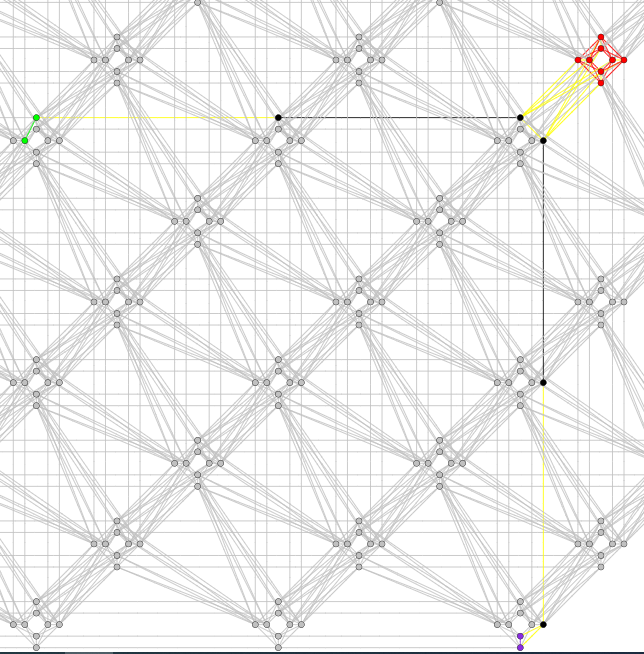
\includegraphics[width=0.95\textwidth]{images/fulladder.PNG}
    \caption{Graphical representation of the fulladder test.}
    \label{fig:my_label}
\end{figure}


\begin{figure}[!]
    \centering
    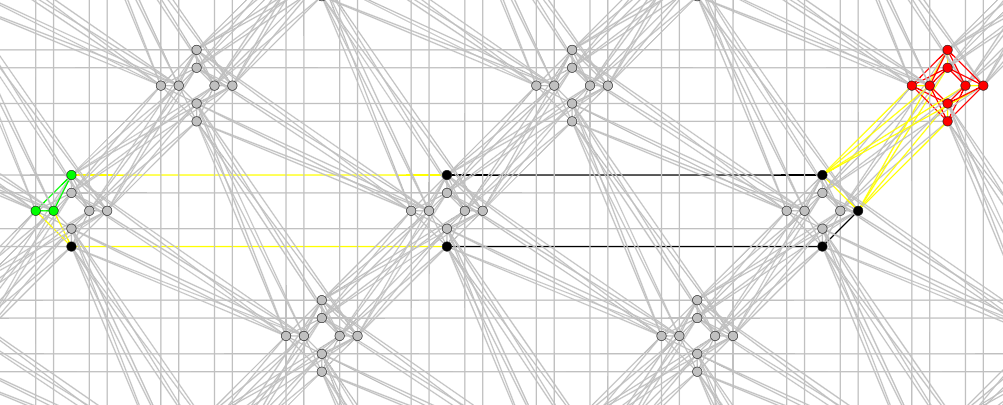
\includegraphics[width=1.0\textwidth]{images/doubleshared.PNG}
    \caption{Graphical representation of the \textit{doublesharing} test.}
    \label{fig:my_label}
\end{figure}

\newpage
\subsection{Testing variation of $min_{gap}$}

This batch of experimental trials will focus on testing the postprocessing procedure using various gates from different complexity, in order to determine if it is actually possible to obtain alternative encodings with higher gaps for a subset of penalty functions. In particular we will test Boolean formulas requiring a number of qubits in a range between 4 to 8 variables, all of them extracted from the old Chimera genlib (opportunely converted into a valid Pegasus formulation). We will first test two cases with a single gate from Chimera genlib, focusing on the increase of $min_{gap}$; next we will try a case where two complex subformulas are involved, simultaneously testing the correctness of the procedure and the  \\

\clearpage

\subsubsection{Gate22}

The two sub-formulas involved into the test case are:

\begin{itemize}
    \item F1 (\textit{gate22}): $o1 = (i1 \vee i2) \wedge (i1 \vee i3) \wedge (i2 \vee i3)$
    \item F2: $i1 \neq e1$
\end{itemize}

Figure 6.3 and table 6.3 report the result of the SAT-To-Ising transformation.

\begin{figure}[hbt!]
    \centering
    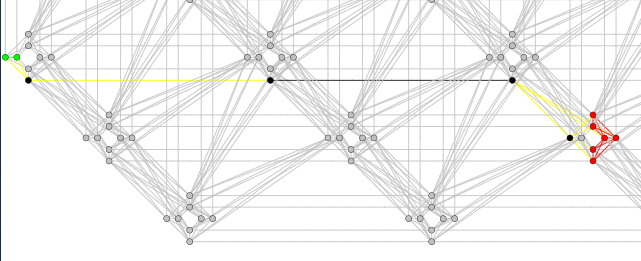
\includegraphics[width=1.0\textwidth]{images/gate22.PNG}
    \caption{Graphical representation of the \textit{gate22} test.}
    \label{fig:my_label}
\end{figure}

\begin{table}[!hbt]
\centering
\begin{tabular}{|c|c|c|}
\hline
 & \cellcolor[HTML]{FFFE65}Classic encoding & \cellcolor[HTML]{FFFE65}Postprocessing encoding \\ \hline
\cellcolor[HTML]{00D2CB}Average chain length & 4 & 1 \\ \hline
\cellcolor[HTML]{00D2CB}N. wasted qubits & 4 & 2 \\ \hline
\cellcolor[HTML]{00D2CB}Max min\_gap & 2 & 4 \\ \hline
\rowcolor[HTML]{67FD9A} 
\cellcolor[HTML]{00D2CB}Correct solution     & Yes                                      & Yes                                             \\ \hline
\end{tabular}
\caption{Evaluation of postprocessing in the \textit{gate22} test}
\end{table}

\newpage

\subsubsection{Gate20}

The two sub-formulas involved into the test case are:

\begin{itemize}
    \item F1 (\textit{gate20}): $o1 = (\neg i1 \vee \neg i2) \wedge (\neg i3)$
    \item F2: $i1 \neq e1$
\end{itemize}

Figure 6.3 and table 6.3 report the result of the SAT-To-Ising transformation.

\begin{figure}[hbt!]
    \centering
    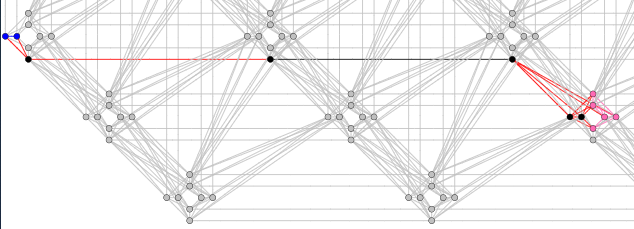
\includegraphics[width=1.0\textwidth]{images/gate20.PNG}
    \caption{Graphical representation of the \textit{gate22} test.}
    \label{fig:my_label}
\end{figure}

\begin{table}[!hbt]
\centering
\begin{tabular}{|c|c|c|}
\hline
 & \cellcolor[HTML]{FFFE65}Classic encoding & \cellcolor[HTML]{FFFE65}Postprocessing encoding \\ \hline
\cellcolor[HTML]{00D2CB}Chain length & 6 & 1 \\ \hline
\cellcolor[HTML]{00D2CB}N. wasted qubits & 5 & 1 \\ \hline
\cellcolor[HTML]{00D2CB}Max min\_gap & 2 & 4 \\ \hline
\rowcolor[HTML]{67FD9A} 
\cellcolor[HTML]{00D2CB}Correct solution     & Yes                                      & Yes                                             \\ \hline
\end{tabular}
\caption{Evaluation of postprocessing in the \textit{gate22} test}
\end{table}

\newpage

\section{Testing benchmark files}

After the verification on simple Boolean problems, we decided to check performances on a small subset of benchmark problems. The main goal was checking how postprocessing impacted the structure of chains and the interconnection among penalty functions, and thus determining how much we could amortize the effect of co-tunneling. Given the limitations of the current Pegasus architectures (in particular the limited number of Boolean variables of the SAT problem so that), the list of suitable test files is quite restricted. Nevertheless, the available files were enough to show the effectivness of the novel approach and have been used in the following tests. The benchmarks we choose for this phase are all listed in \cite{aiger}. The concerns:

\begin{itemize}
    \item \textbf{c17}, the first file from the \textit{ISCAS} benchmark representing a 6-NAND-gate circuit.
    \item \textbf{bj08aut1}, \textbf{pdtvisgray0} and \textbf{pdtvisgray1} coming from the Hardware Model Checking Competition 2008. They have been tested on Pegasus6.
    \item \textbf{nusmvsyncarb5p2} coming from the Hardware Model Checking Competition 2010. They have been tested in Pegasus12.
\end{itemize}

We tested both the original algorithm and the postprocessing to the mentioned files, obtaining in both cases valid assignments. Statistics about the average length of chains is shown in table 6.5.

\begin{table}[hbt!]
\centering
\begin{tabular}{|c|c|c|}
\hline
                                    & \cellcolor[HTML]{FFFE65}Average chain length: old version & \cellcolor[HTML]{FFFE65}Average chain length: postprocessing \\ \hline
\cellcolor[HTML]{00D2CB}bj08aut1    & 5.444                                                     & 3.389                                                        \\ \hline
\cellcolor[HTML]{00D2CB}pdtvisgray0 & 5.0625                                                    & 2.5625                                                       \\ \hline
\cellcolor[HTML]{00D2CB}pdtvisgray1 & 5.133                                                     & 2.733                                                        \\ \hline
\cellcolor[HTML]{00D2CB}c17         & 3.923                                                     & 2.923                                                        \\ \hline
\cellcolor[HTML]{00D2CB}nusmvsyncarb5p2 & 4.07 & 2.282
\end{tabular}
\caption{Evaluation of the postprocessing algorithm on some benchmark files with respect to the average length of chains}
\end{table}


\newpage

